\section{Rotations and Minimal Differences}

In this section, we will exhibit a one-one correspondence between the rotations and the minimal differences of $\mathrm{P}(\mathcal{M})$. Then, given Lemma \ref{lem_3_2} and Lemma \ref{lem_3_3} above, and the fact that all the minimal differences are found along any maximal chain of $P(\mathcal{M})$, we will be able to identify all the minimal differences and all the rotations by successively finding and eliminating exposed rotations, myopicly following any maximal chain in $\mathcal{M}$ from $M_0$ to $M_z$. The following is a central technical lemma.

\begin{lemma}\label{lem_3_5}
If $M$ strictly dominates $M^{\prime}$, and $\rho$ is exposed in $M$, then either all the men in $\rho$ have the same partners in $M$ and in $M^{\prime}$, or none of them does. In the latter case, $M / \rho$ dominates $M^{\prime}$. Similarly, if a man $m$ is on a tail of $\rho$, and $m$ has different partners in the two matchings, then so does every man in $\rho$, and again $M / \rho$ dominates $M^{\prime}$.
\end{lemma}

\begin{proof}
By Lemma \ref{lem_3_1}, if $m_i \in \rho$ has a different partner $w$ in $M^{\prime}$ than in $M$, then $w$ must either be $s_M\left(m_i\right)$ or a woman below her in $m_i$ 's list. In either case, $s_M\left(m_i\right)$ must not be matched in $M^{\prime}$ to $m_{i+1}$, her partner in $M$, for if $s_M\left(m_i\right)$ and $m_{i+1}$ are partners in $M^{\prime}$, then either $s_M\left(m_i\right)$ has two partners in $M^{\prime}$, or the pair $\left(m_i,s_M\left(m_i\right)\right)$ blocks $M^{\prime}$. Hence $m_{i+1}$ must also have a different partner in $M^{\prime}$ than in $M$, and it follows that all men in $\rho$ have different partners in $M$ and $M^{\prime}$ if any one of them does. In the case that the men of $\rho$ have different partners in the two matchings, Lemma \ref{lem_3_1} implies that $M / \rho$ dominates (possibly equals) $M^{\prime}$, since the only men with different partners in $M$ and $M / \rho$ are the men in $\rho$. The case when $m$ is on a tail of $\rho$ is proved in essentially the same way, using Lemma \ref{lem_3_4} in place of Lemma \ref{lem_3_1}.
\end{proof}

\begin{exmp}\label{exmp_3_5}
In Figure \ref{FIG_2_2}, $M_1$ dominates both $M_4$ and $M_5$, among other matchings, and the rotation $(1,8),(2,3),(4,6)$, which we will call $\rho_1$, is exposed in $M_1$. In matching $M_5$, every man in $\rho_1$ has the same partner he has in $M_1$, while in $M_4$ every man in $\rho_1$ has a different partner. Further, $M_2=M_1 / \rho_1$ and $M_2$ dominates $M_4$, as required by the lemma.
\end{exmp}

\begin{theorem}\label{thm_3_1}
If $\rho$ is exposed in $M$, then $M$ is an immediate predecessor of $M / \rho$ in $\mathcal{M}$, and $P(M / \rho) \backslash P(M)$ is a minimal difference of $P(\mathcal{M})$.
\end{theorem}

\begin{proof}
    It is immediate from Lemma \ref{lem_3_5} that there is no stable matching $M^{\prime}$ such that $M$ dominates $M^{\prime}$, and $M^{\prime}$ dominates $M / \rho$, so $M$ immediately precedes $M / \rho$. Then by Lemma \ref{lem_2_11}, $P(M / \rho) \backslash P(M)$ is a minimal difference of $P(\mathcal{M})$.
\end{proof}

For rotation $\rho=\left(m_0, w_0\right),\left(m_1, w_1\right), \ldots,\left(m_{r-1}, w_{r-1}\right)$, we define $d(\rho)$ to be the set all pairs $\left(m_i, w\right)$, where $m_i \in \rho$ and $w$ is either $w_{i+1}$ or a woman strictly between $w_i$ and $w_{i+1}$ in $m_i$ 's list.

\begin{exmp}\label{exmp_3_6}
    When $\rho=(3,5),(6,1)$, which is a rotation in the example from Figure \ref{FIG_2_2}, then $m_0=3, m_1=6, w_0=5, w_1=1$, and so it can be seen from the preference lists of Figure \ref{FIG_2_1} that $d(\rho)=\{(3,1),(6,6),(6,7),(6,5)\}$
\end{exmp}

Notice that rotation $\rho$ is completely determined by the set of pairs $d(\rho)$ and the preference lists, and that $\rho$ can be constructed from $d(\rho)$ as follows: for each man $m$ in a pair $(m, w) \in d(\rho)$, let $w(m)$ be the woman $m$ most prefers among the women $w$ such that $(m, w)$ is in $d(\rho)$; let $\hat{w}(m)$ be the woman immediately before $w(m)$ in $m$ 's preference list. Then $\rho$ consists of all pairs $(m, \hat{w}(m))$, such that $m$ is in a pair $(m, w) \in d(\rho)$. The order of the pairs in $\rho$ is easily determined from these pairs and the preference lists.

\begin{lemma}\label{lem_3_6}
    If rotation $\rho$ is exposed in distinct matchings $M$ and $M^{\prime}$, then $P(M / \rho) \backslash P(M)=$ $P\left(M^{\prime} / \rho\right) \backslash P\left(M^{\prime}\right)=d(\rho)$.
\end{lemma}

\begin{proof}
    The difference $P(M / \rho) \backslash P(M)$ consists of all pairs $\left(m_i, w\right)$, where $w$ is either $w_{i+1}$ or a woman strictly between $w_i$ and $w_{i+1}$ in $m_i$ 's list. Clearly this set of pairs depends only on $\rho$ and the preference lists, and not on $M$. Hence, $P(M / \rho) \backslash P(M)=P\left(M^{\prime} / \rho\right) \backslash P\left(M^{\prime}\right)$, and they both are $d(\rho)$.
\end{proof}

Combining Lemma \ref{lem_3_6} and Theorem \ref{thm_3_1}, we have the following.

\begin{theorem}\label{thm_3_2}
    For any rotation $\rho$, the set of pairs $d(\rho)$ is a minimal difference of $P(\mathcal{M})$, and so each rotation $\rho$ maps to a unique minimal difference $d(\rho)$. Further, $d(\rho)$ can be constructed directly from $\rho$ and the preference lists.
\end{theorem}

%\begin{theo}
\begin{center}
\begin{minipage}{.8\linewidth}
\begin{algorithm}[H]
\caption{\textit{Minimal-differences}}
\begin{algorithmic}[1]
\State find the man and the woman-optimal matchings $M_0$, $M_z$;
\State $i:= 0$
\While {$M_i \neq M_z$}
\State Find an exposed rotation $\rho \in M_{i}$
\State $M_{i+1} := M_i/\rho_i$
\State $d(\rho_i) := P(M_{i+1}) \ P(M_i)$;
\EndWhile
\end{algorithmic}
\end{algorithm}
\end{minipage}

\begin{figure}[ht]
  \centering
  \caption{Algorithm to fnd all the minimal differences and rotations}
  \label{FIG_3_4}
\end{figure}
\end{center}
%\end{theo}

Our goal now is to show the converse of Theorem \ref{thm_3_2}, i.e., that every minimal difference of $P(\mathcal{M})$ is $d(\rho)$ for exactly one rotation $\rho$. We will do this through the use of Algorithm minimal differences, shown in Figure \ref{FIG_3_4}. This algorithm will find all the minimal differences of $P(\mathcal{M})$, and all the rotations of $\mathcal{M}$, using only the preference lists of the problem instance.

\begin{theorem}\label{thm_3_3}
    Every minimal difference of $P(\mathcal{M})$ is the set $d(\rho_i)$ for exactly one rotation $\rho_i$ generated by Algorithm minimal-differences and every rotation in $\mathcal{M}$ is generated exactly once by Algorithm minimal-differences.
    
\end{theorem}



\begin{proof}
    By Lemmas 2.5.2 and 2.5.3, each $M_i$ generated by the algorithm is a stable matching, and there is an exposed rotation in each matching until the woman optimal matching is reached. Further, by Theorem \ref{thm_3_1}, each $M_i$ is an immediate predecessor in $\mathcal{M}$ of $M_{i+1}$. Hence the sequence of st able matchings generated by the algorithm must be a maximal chain in $\mathcal{M}$ from the man optimal matching to the woman optimal matching. Now by Corollary \ref{cor_2_5}, every minimal difference of $\mathcal{M}$ appears exactly once as a consecutive difference of matchings along any maximal chain in $\mathcal{M}$; hence, every minimal difference of $\mathcal{M}$ is $d\left(\rho_i\right)$ for exactly one $\rho_i$ generated by the algorithm.
\end{proof}

For the second claim, let $\rho$ be any rotation, and let $M$ be any stable matching in which it is exposed. By Lemma \ref{lem_3_6} $d(\rho)=P(M / \rho) \backslash P(M)$, which is a minimal difference, by Theorem \ref{thm_3_1}. Hence $d(\rho)=d\left(\rho_i\right)$, for some $\rho_i$ found by the algorithm. But since $d(\rho)$ uniquely determines $\rho$, it follows that $\rho=\rho_i$.

Lets say that a rotation $\rho$ is on a chain in $\mathcal{M}$, and that the chain contains $\rho$, if the minimal difference $d(\rho)$ is on the corresponding chain in $P(\mathcal{M})$. Then, combining the results of this section with Theorem \ref{thm_2_1} we have the main result of this section.

\begin{theorem}\label{thm_3_4}
    There is a one-one correspondence $\rho \leftrightarrow d(\rho)$ between the rotations of $\mathcal{M}$ and the minimal differences of $P(\mathcal{M})$. Further, if $M$ dominates $M^{\prime}$, then every chain in $\mathcal{M}$ between $M$ and $M^{\prime}$ contains exactly the same set of rotations. Hence every rotation of $\mathcal{M}$ appears exactly once on every maximal chain of $\mathcal{M}$.
\end{theorem}
    
\begin{exmp}\label{exmp_3_7}
    Lets demonstrate Algorithm minimal-differences on the problem instance shown in Figure \ref{FIG_2_1}. In the example, we will use reduced preference lists. This will keep the lists smaller, and make it easier to recognize exposed rotations. Also, we will display only the reduced lists of the men, as all information can be extracted from their reduced lists. To verify that the reduced lists of the men are maintained correctly. To start, the $MGS$-lists for the man-optimal matching $M_0$ are shown in Figure \ref{FIG_3_5} 
\end{exmp}

\begin{center}
    $\begin{array}{llllllll}1: & 5 & 8 & 3 & & & & \\ 2: & 3 & 8 & 6 & & & & \\ 3: & 8 & 5 & 1 & 6 & 2 & & \\ 4: & 6 & 8 & 5 & & & & \\ 5: & 7 & 2 & 1 & 3 & 6 & 8 & 4 \\ 6: & 1 & 5 & 2 & 3 & & & \\ 7: & 2 & 5 & 7 & 8 & 1 & & \\ 8: & 4 & 5 & 2 & 6 & & & \end{array}$
    \begin{figure}[h]
  \centering
  \caption{ The $MGS$ lists}
  \label{FIG_3_5}
\end{figure}
\end{center}

\begin{exmp}\label{exmp_3_8}
    There is one exposed rotation $\rho_0=(1,5),(3,8)$ in $M_0$, and $M_0 / \rho_0=M_1$. The reduced lists for $M_1$ were used in an earlier example and appear in Figure \ref{FIG_3_2}. As noted before, there are two exposed rotations in $M_1$. Suppose the algorithm picks rotation $\rho_1=(1,8),(2,3),(4,6)$ at this point. Then $M_1 / \rho_1=M_2$; the reduced lists of the men for $M_2$ are shown in Figure \ref{FIG_3_6} .
\end{exmp}


\begin{exmp}\label{exmp_3_9}
    In $M_2$ there is one exposed rotation, $\rho_2=(3,5),(6,1)$, and $M_2 / \rho_2=M_4$ (note that we are using the name of the matching given in Figure \ref{FIG_2_2} rather than the name given by Algorithm minimal-differences). The reduced lists for $M_4$ are shown in Figure \ref{FIG_3_7}.
\end{exmp}

\begin{exmp}\label{exmp_3_10}
    The rotation $\rho_3=(7,2),(5,7)$ is exposed in $M_4$, and $M_4 / \rho_3=M_6$. The reduced lists are shown in Figure \ref{FIG_3_8}.
\end{exmp}

\begin{exmp}\label{exmp_3_11}
    Rotation $\rho_4=(3,1),(5,2)$ is exposed in $M_6$, and $M_6 / \rho_4=M_7$, the woman-optimal matching. The final reduced lists are shown in Figure \ref{FIG_3_9}.
\end{exmp}



\begin{center}
    $\begin{array}{llllll}1: & 3 & & & & \\ 2: & 6 & & & & \\ 3: & 5 & 1 & 2 & & \\ 4: & 8 & 5 & & & \\ 5: & 7 & 2 & 1 & & \\ 6: & 1 & 5 & 2 & & \\ 7: & 2 & 5 & 7 & 8 & 1 \\ 8: & 4 & 2 & & & \end{array}$
    \begin{figure}[ht]
  \centering
  \caption{The reduced lists of the men for stable matching $M_2$}
  \label{FIG_3_6}
\end{figure}
\end{center}


\begin{center}
    $\begin{array}{llll}1: & 3 & & \\ 2: & 6 & & \\ 3: & 1 & 2 & \\ 4: & 8 & & \\ 5: & 7 & 2 & 1 \\ 6: & 5 & 2 & \\ 7: & 2 & 7 & 8 \\ 8: & 4 & 2 & \end{array}$
    \begin{figure}[ht]
  \centering
  \caption{The reduced lists of the men for stable matching $M_4$}
  \label{FIG_3_7}
\end{figure}
\end{center}

\begin{center}
    $\begin{array}{lll}1: & 3 & \\ 2: & 6 & \\ 3: & 1 & 2 \\ 4: & 8 & \\ 5: & 2 & 1 \\ 6: & 5 & 2 \\ 7: & 7 & 8 \\ 8: & 4 & 2\end{array}$
    \begin{figure}[ht]
  \centering
  \caption{The reduced lists of the men for stable matching $M_6$}
  \label{FIG_3_8}
\end{figure}
\end{center}

\begin{center}
    $\begin{array}{lll}1: & 3 & \\ 2: & 6 & \\ 3: & 2 & \\ 4: & 8 & \\ 5: & 1 & \\ 6: & 5 & 2 \\ 7: & 7 & 8 \\ 8: & 4 & 2\end{array}$
    \begin{figure}[ht]
  \centering
  %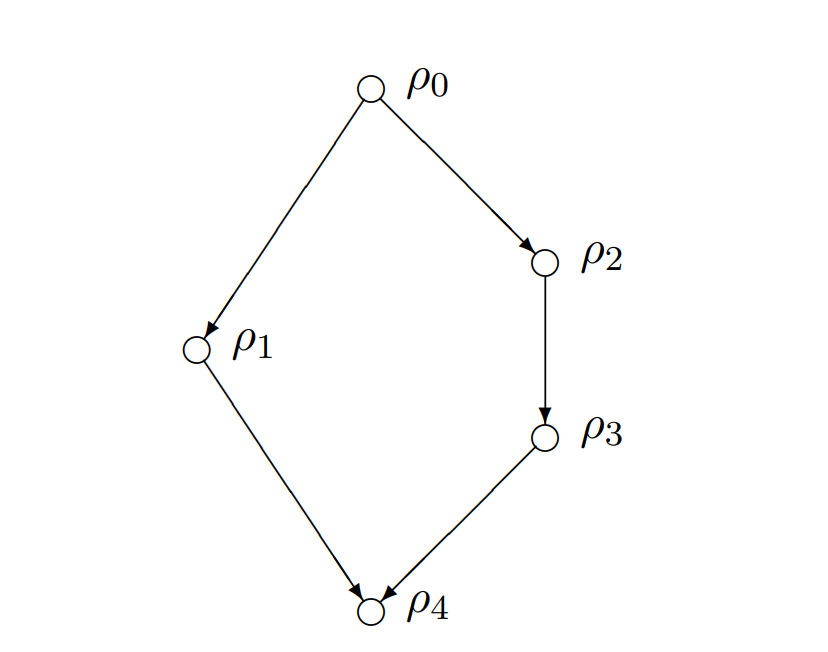
\includegraphics[width=0.5\textwidth]{IMAGES_FIGS/FIG_2_8.png}
  \caption{The reduced lists of the men for woman-optimal matching}
  \label{FIG_3_9}
\end{figure}
\end{center}



Even without additional implementation detail, it is easy to establish that Algorithm minimal differences needs no more than $O\left(n^3\right)$ time to find all the rotations. In the next chapter we will implement Algorithm minimal-differences to run in $O\left(n^2\right)$ time.

Any stable matching $M$ other than $M_z$ has an exposed rotation $\rho$ that defines a minimal difference $d(\rho)$, and both $\rho$ and $d(\rho)$ are easy to find from the reduced lists for $M$. Hence rotations allow one to focus on a single stable matching $M$, knowing that $d(\rho)$ is a minimal difference of $\mathcal{M}$, whereas the definition of a minimal difference involves a very particular stable matching, an irreducible one, or involves two stable matchings. The existence of rotations is the special, algorithmically valuable feature of $P(\mathcal{M})$ that does not exist in a general ring of sets.
